\documentclass{standalone}
\usepackage{picture,color}
\usepackage{graphicx}
\graphicspath{{./all_scans_block_0_raw/}}
\setlength{\unitlength}{1in}
\renewcommand{\rmdefault}{phv} 
\renewcommand{\sfdefault}{phv} 

\begin{document}
\begin{picture}(5.65, 5.46)(0.09,-5.46)
%good em ids: 
%23683777
% raw data 
\put(4.02, -3.2){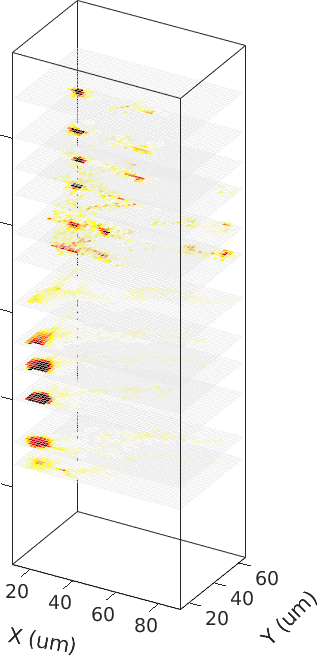
\includegraphics[height=3in]{EM_23683777_2p_3d.png}}
\put(2.2, -3.2){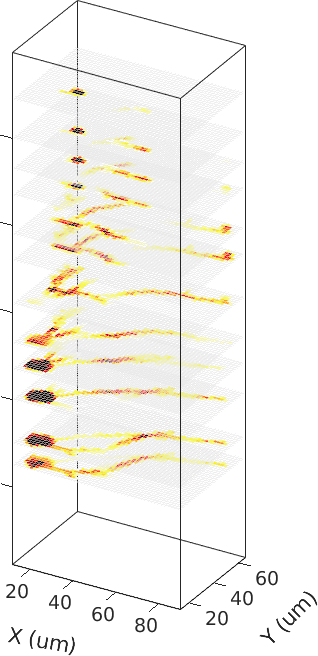
\includegraphics[height=3in]{EM_23683777_em_3d.png}}
\put(0.1, -3.2){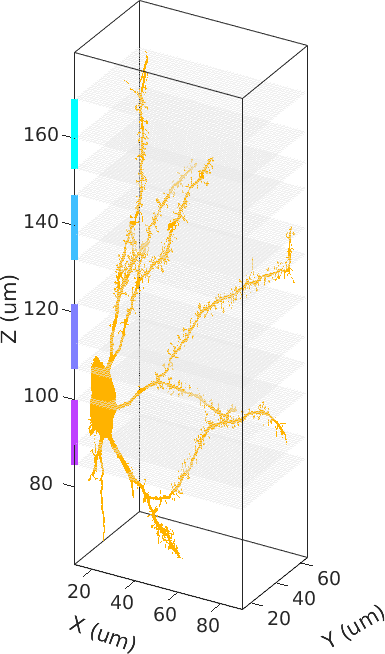
\includegraphics[height=3in]{EM_23683777_meshes_3d.png}}

\put(0.1, -0.25){\large\textbf{A}}
\put(2.1, -0.25){\large\textbf{B}}
\put(3.92, -0.25){\large\textbf{C}}

\put(.7, -0.17){EM mesh}
\put(2.48, -0.17){EM footprint}
\put(4.3, -0.17){2P footprint}

\put(4.03, -5.45){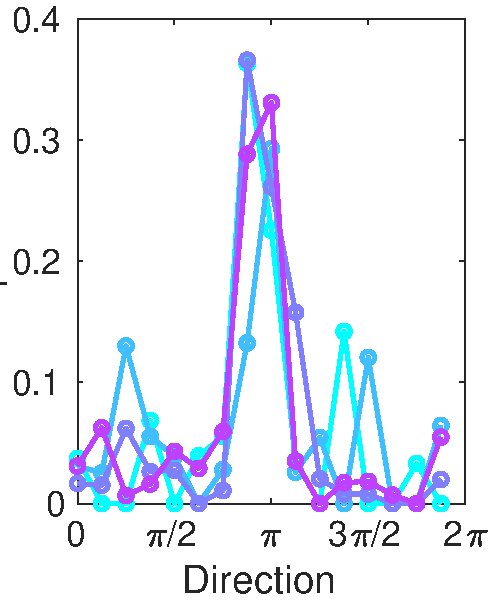
\includegraphics[height=2.1in]{EM_23683777_tuning_curve.pdf}}
\put(4.53, -3.38){Tuning Curves}
\put(4.03, -3.4){\large\textbf{E}}
\put(0.15, -5.24){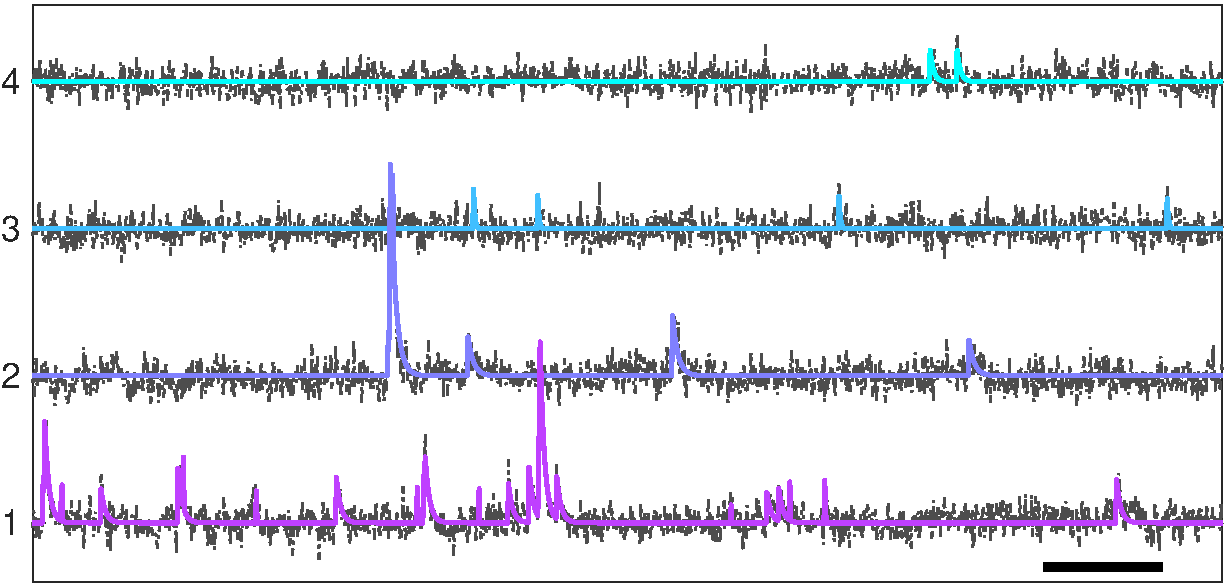
\includegraphics[height=1.83in]{EM_23683777_traces.pdf}}
\put(0.1, -3.4){\large\textbf{D}}

% \put(0.1, -3.3){\large\textbf{E}}
\end{picture}
\end{document}
